\section{在室者状況の提示方法に関する研究}\label{2.3}
在室者を検出した後に在室者情報を用いた在室者状況の提示方法は様々ある
\cite{picture}
\cite{iptelephone}
\cite{staycomment}
\cite{kasika}
\cite{zaiseki}.
利用者全員が見られるサイネージに在室者情報を提示するものや,個人が所有しているスマートフォンやタブレットから在室状況を確認できるものなどがある.
サイネージに提示する手法を用いた研究を図\ref{staystate}\cite{kasika},図\ref{stayniwatori}\cite{kasika}に示す.
利用者全員が見られるサイネージに提示する手法では,一目で在室情報を確認できる必要がある.
スマートフォンやタブレットに提示する手法を用いたものを図
\ref{zaiseki}
% \cite{zaiseki}
に示す.
また個人が所有しているスマートフォンやタブレットから在室状況を確認できる手法ではスマートフォンやタブレットに適するレイアウトを考える必要がある.
本研究ではその場にいる人のコミュニケーション促進するために,その場にいる人が見られるサイネージに提示する手法を採用した.
% \begin{figure}[H]
%   \begin{center}
%     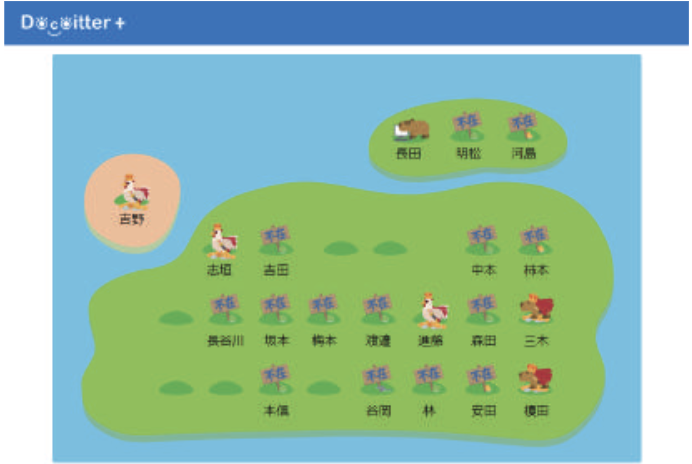
\includegraphics[width=160mm]{image/staystate.png}
%     \caption{在室状況を提示している画面\cite{kasika}}
%     \label{staystate}
%   \end{center}
% \end{figure}
% \begin{figure}[H]
%   \begin{center}
%     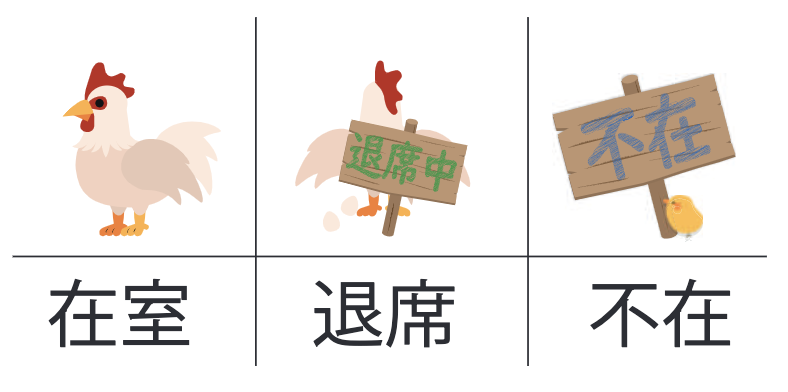
\includegraphics[width=100mm]{image/stayniwatori.png}
%     \caption{在室状況のアバタ例\cite{kasika}}
%     \label{stayniwatori}
%   \end{center}
% \end{figure}
% \begin{figure}[H]
%   \begin{center}
%     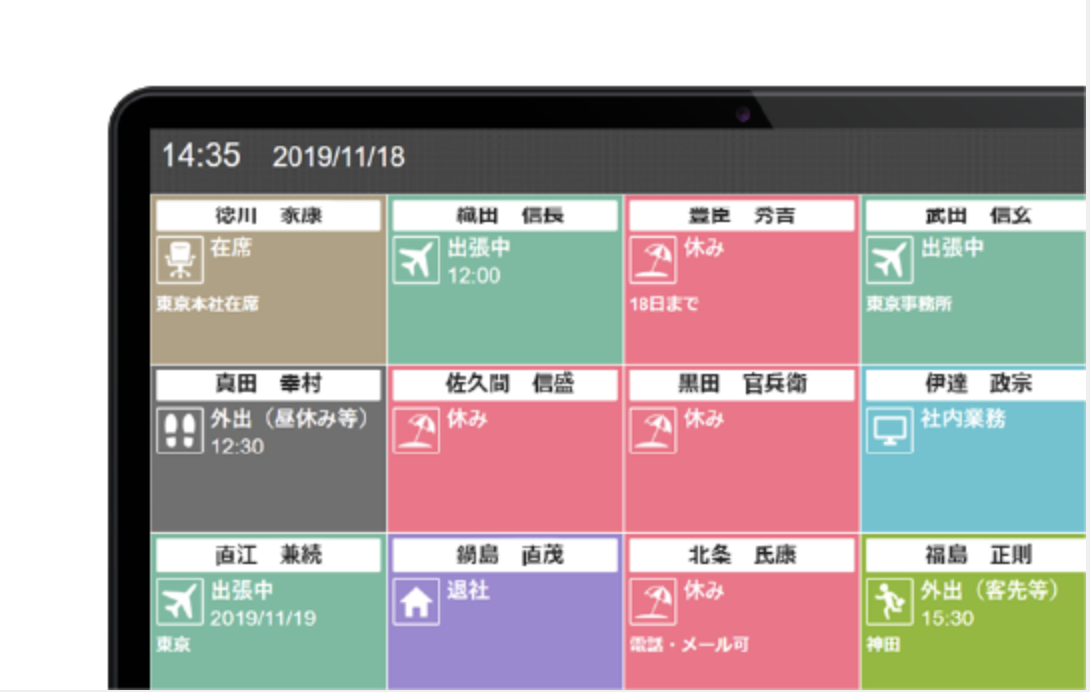
\includegraphics[width=150mm]{image/zaiseki.png}
%     \caption{テレワーク時の所在管理\cite{zaiseki}}
%     \label{zaiseki}
%   \end{center}
% \end{figure}

